
\section{Object identification}
The pipeline is usually invoked by running a single command on a night's worth of data. For example, to build the light-curves for the night of, say, \emph{2014-08-21}, then a single command, \texttt{daybuilder.py 2014-08-21} is issued from the command line. The pipeline then runs through all of the data for that night and generates a set of web pages. Depending on the amount of data for that night, this can take 1 hour to 8 hours. 

For each night, an index page, which shows a list of all of the runs in the night along with thumbnail images of the field of view, is created. This allows the user to quickly navigate to the runs that are of interest. In other words, runs that contain science data, rather than acquisitions, biases or flat-fields. By clicking on the thumbnail of the run, the user is taken to a run page. This page shows the full image for each of the three channels. These images are created by stacking all of the individual frames in the run. The page also shows all of the objects that have been identified and have light-curves available. The user can view the light-curves by using the mouse to click on each object, or can scroll through all of the light-curves systematically, by using the left and right arrow keys. 

Scrolling through the light curves in a systematic fashion makes it easy for the user to quickly identify which objects are showing an obvious variability. All of the objects listed below were discovered in this way. 

The task is made relatively easy in the browser interface and it is possible to inspect the light curves at a rate of about 1-2 objects per second. In future, we plan to apply some automated tests to these data to perform the light curve inspection as an integral stage of the automated pipeline. Algorithms to perform these sorts of tests are already known and becoming increasingly more widespread as more large scale sky surveys are being used throughout astronomy research. We plan to re-use work from one or more of these surveys. The recently published Astrokit software, (\cite{Astrokit2014}) is one tool that we plan to trial in the next version of the automated pipeline. 

\emph{Comment: References to VVV, LSST, NGTS, Wasp,  etc.}

\section{Discovered objects}
As discussed in the introduction, chapter \ref{chap:introduction}, we expect to find some new variables in the ULTRACAM archive. These will be objects displaying some kind of variability that is clearly visible over the length of the run and the cadence of the observations. The kinds of objects that should be clear will include eclipsing binaries, contact binaries, flare stars, RR Lyrae and $\delta$ Scuti stars. We might also expect to see other short period variables like cataclysmic variables and DV white dwarfs. Since the pipeline is able to track slow moving objects, we can also expect that we will capture photometry of asteroids.   

So far, we have only inspected approximately 20\% of the reduced data but we have have a few dozen variable objects
Below we list some of the variable objects that have discovered as a result of running the automated pipeline on a fraction of the ULTRACAM archive. 

\newpage
\subsection{Eclipsing binaries}

  \begin{figure}
    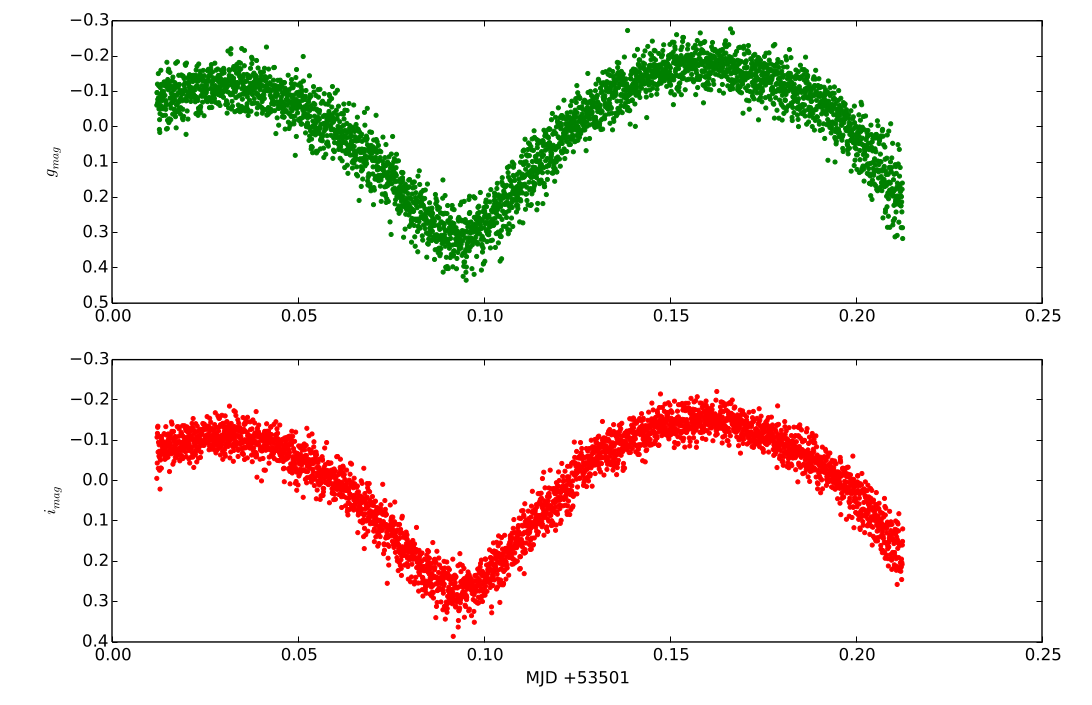
\includegraphics[width=120mm]{images/2005-05-10-run012-73-lightcurve-cropped.png} 
    \label{fig:2005-05-10-run012}
    \caption{Sloan i and g light curves of object: 2005-05-10-run012-73}
  \end{figure}
  
  \begin{tabular}{l l}
  Classification & {W UMa} contact binary \\
  Original target & GU Mus \\
  ObjectID & 2005-05-10-run012-73 \\
  RA, DEC & 19:44:09.8, 40:16:34.4 (J2000) \\
  Run date & 2005-05-10 \\
  Pixel position & (232, 65) \\
  %URL: & \small \url{http://deneb.astro.warwick.ac.uk/phrnaw/sitedev/2005-05-10/run012.html} \\
   & 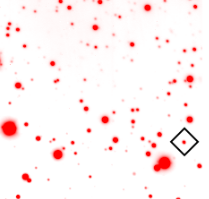
\includegraphics[width=40mm]{images/2005-05-10-run012-73.png} \\
  \end{tabular}
  
  The original target of this run was the X-ray transient, {GU Mus}, that was observed in quiescence in 2005. The compact object was accreting at the time and flickering is apparent in the optical light curve in all three of the Sloan i, g, and u bands, (\cite{tariq2010}). About 4 arc minutes to the west we have detected a suspected {W Uma} contact binary with an apparent magnitude of $\sim21$ in Sloan g and period of yy minutes. Visual inspection of the light-curves in figure \ref{fig:2005-05-10-run012} shows evidence of the O'Connell effect where the peak brightness of the second maximum is larger than the first. 

The cause of the O'Connell effect is something that is still debated in astronomy, (\cite{oconnelleffect}). Differences in the brightness of the minima of the light-curves is something that is expected and is caused by the different sizes and temperatures of each component in the system. Based on a geometric model of the eclipse though, we would expect the maxima to be of equal brightness since we are seeing the system `side-on' at both maxima with the same ellipsoidal faces presented to the observer. Current explanations consist of star-spots that are locked in rotational synchronisation with the orbit and are presented preferentially on one side of the system; gas streams in systems that are relatively far apart (contact or near-contact, rather than over-contact); and circumstellar material that might be kinetically heated and gather preferentially on the leading edge of the orbiting bodies.  


% This target has another day of observations. 2005-05-09. The data should be combined, ephemeris found and light curve phase folded. 

\newpage

\begin{figure}
  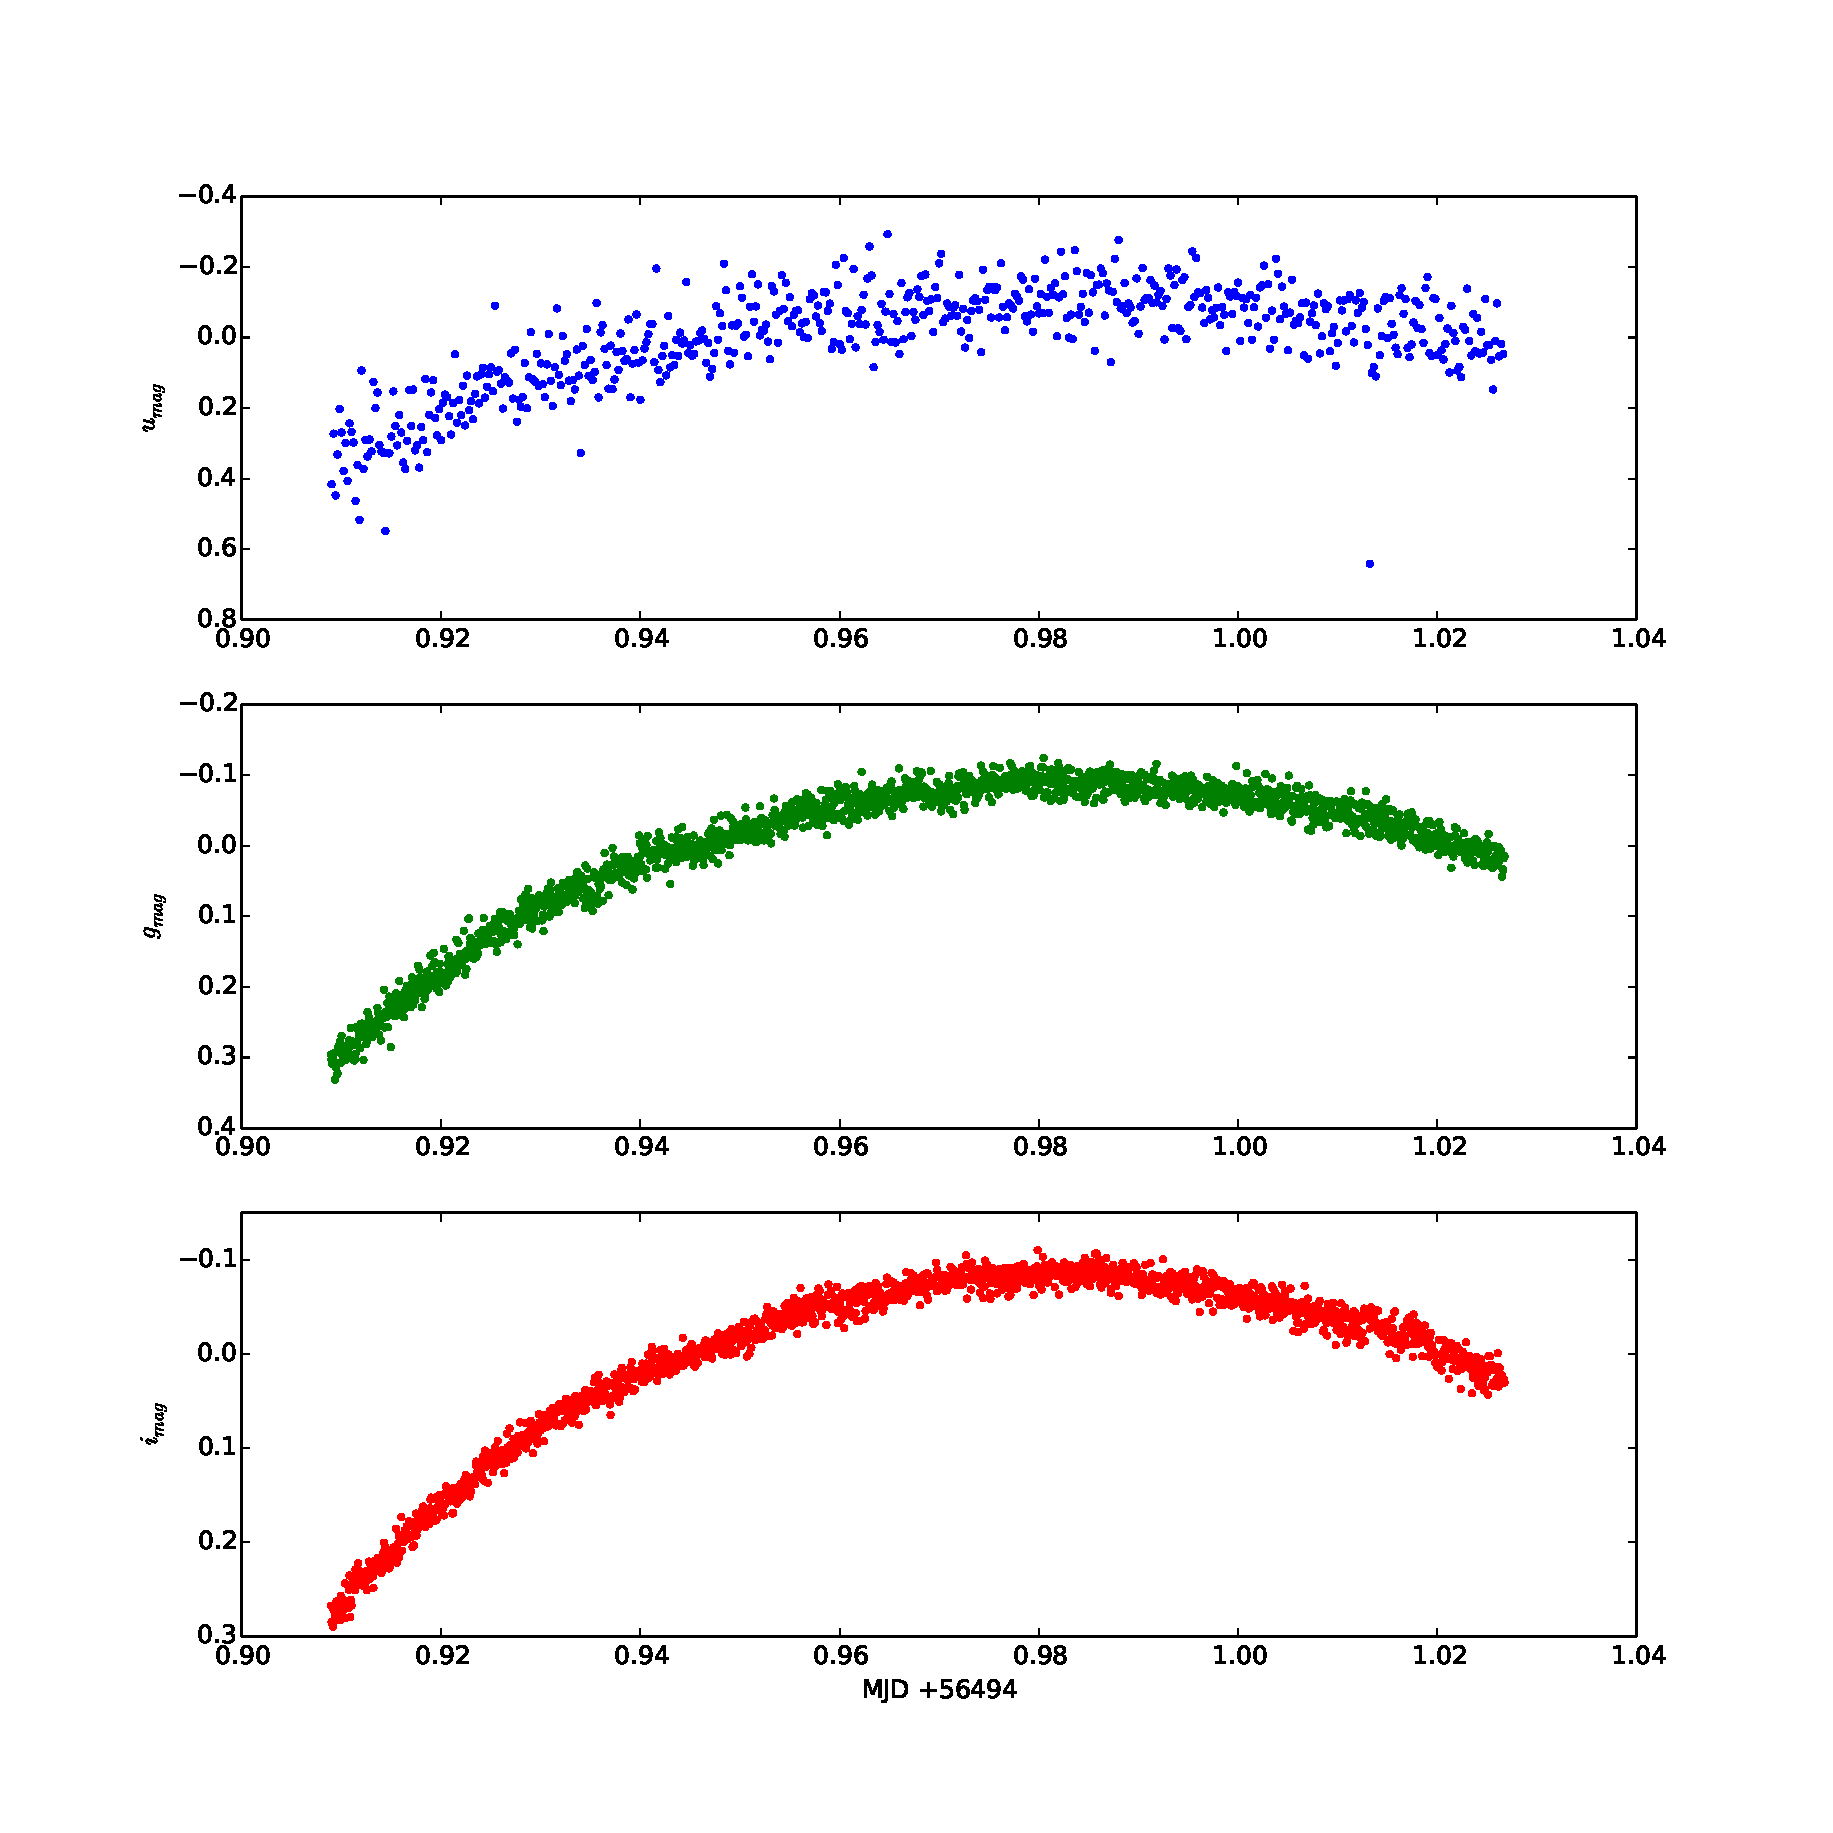
\includegraphics[width=120mm]{images/2013-07-21-run010-48_lightcurve.eps} 
  \label{fig:2005-05-10-run012}
  \caption{Sloan i, g and u light curves of object: 2013-07-21-run010-48}
\end{figure}

  \begin{tabular}{l l}
  Classification & {W UMa} contact binary \\
  ObjectID & 2013-07-21-run010-48 \\
  Original target & J19440167+4017435 also KOI-823 \\
  RA, DEC & 19:44:09.8, 40:16:34.4 (J2000) \\
  Run date & 2013-07-21 \\
  Pixel position & (452, 332) \\
  % URL: & \small \url{http://deneb.astro.warwick.ac.uk/phrnaw/sitedev/2013-07-21/run010.html} \\
       & 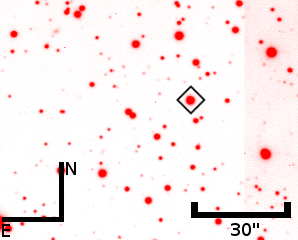
\includegraphics[width=60mm]{images/2013-07-21-run010-48.png} \\
  \end{tabular}
 
  \newpage
  \begin{tabular}{l l}
  Classification & {W UMa} contact binary \\
  ObjectID & 2013-07-21-run010-163 \\
  RA, DEC & 19:44:10.3, 40:18:08.1 (J2000) \\
  Run date & 2013-07-21 \\
  Pixel position & (417, 650) \\
  URL: & \small \url{http://deneb.astro.warwick.ac.uk/phrnaw/sitedev/2013-07-21/run010.html} \\
       & 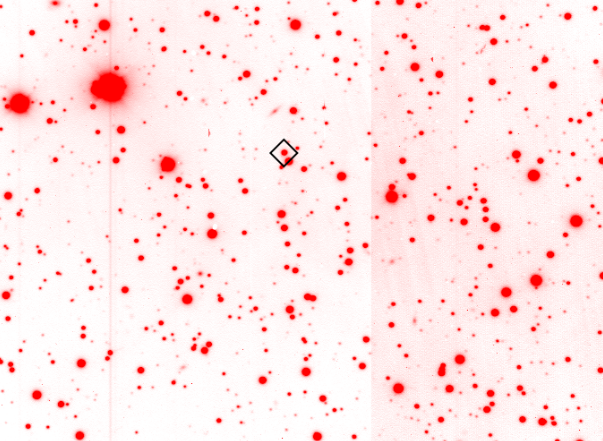
\includegraphics[width=60mm]{images/2013-07-21-run010-163.png} \\
  \end{tabular}
  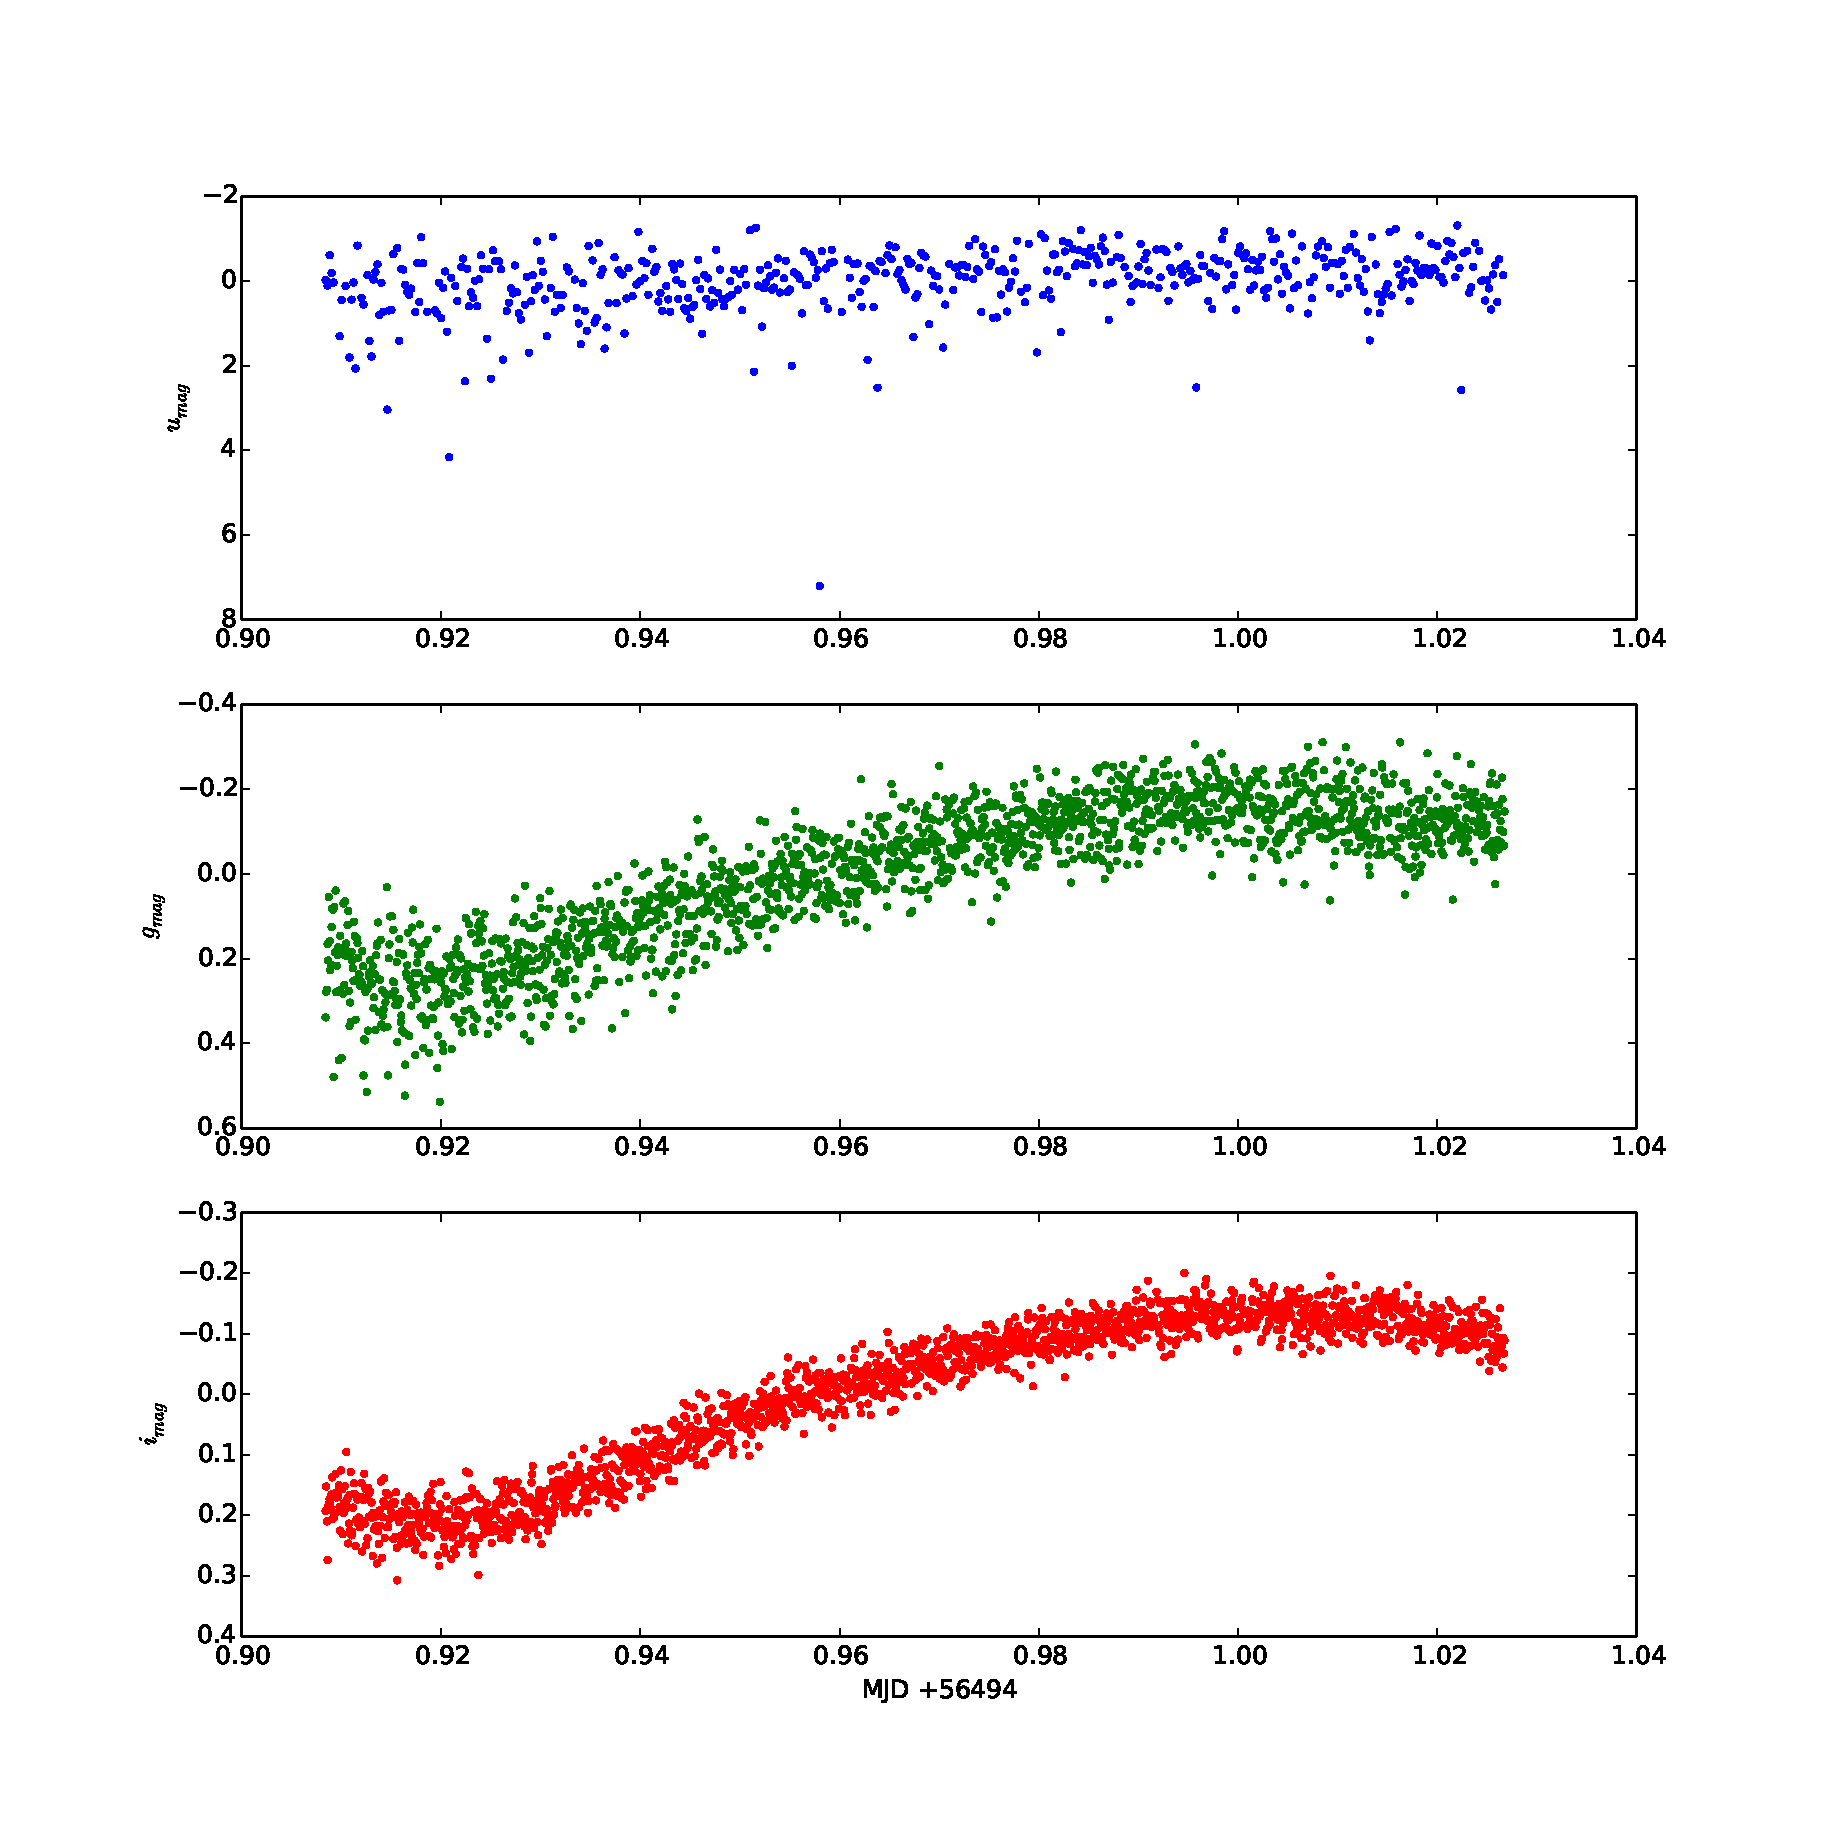
\includegraphics[width=120mm]{images/2013-07-21-run010-163_lightcurve.eps} \\
  Discussion of this object.

  \newpage
  \begin{tabular}{l l}
  Classification & Eclipsing binary \\
  ObjectID & 2013-07-21-run011-162 \\
  Pixel position & (726, 341) \\
  RA, DEC & 19:54:01.7, 40:37:34 (J2000) \\
  URL: & \small \url{http://deneb.astro.warwick.ac.uk/phrnaw/sitedev/2013-07-21/run011.html} \\
       & 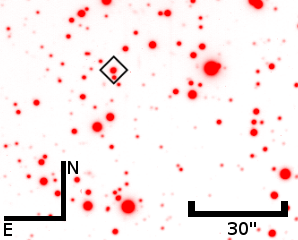
\includegraphics[width=60mm]{images/2013-07-21-run011-162.png} \\
  \end{tabular}
  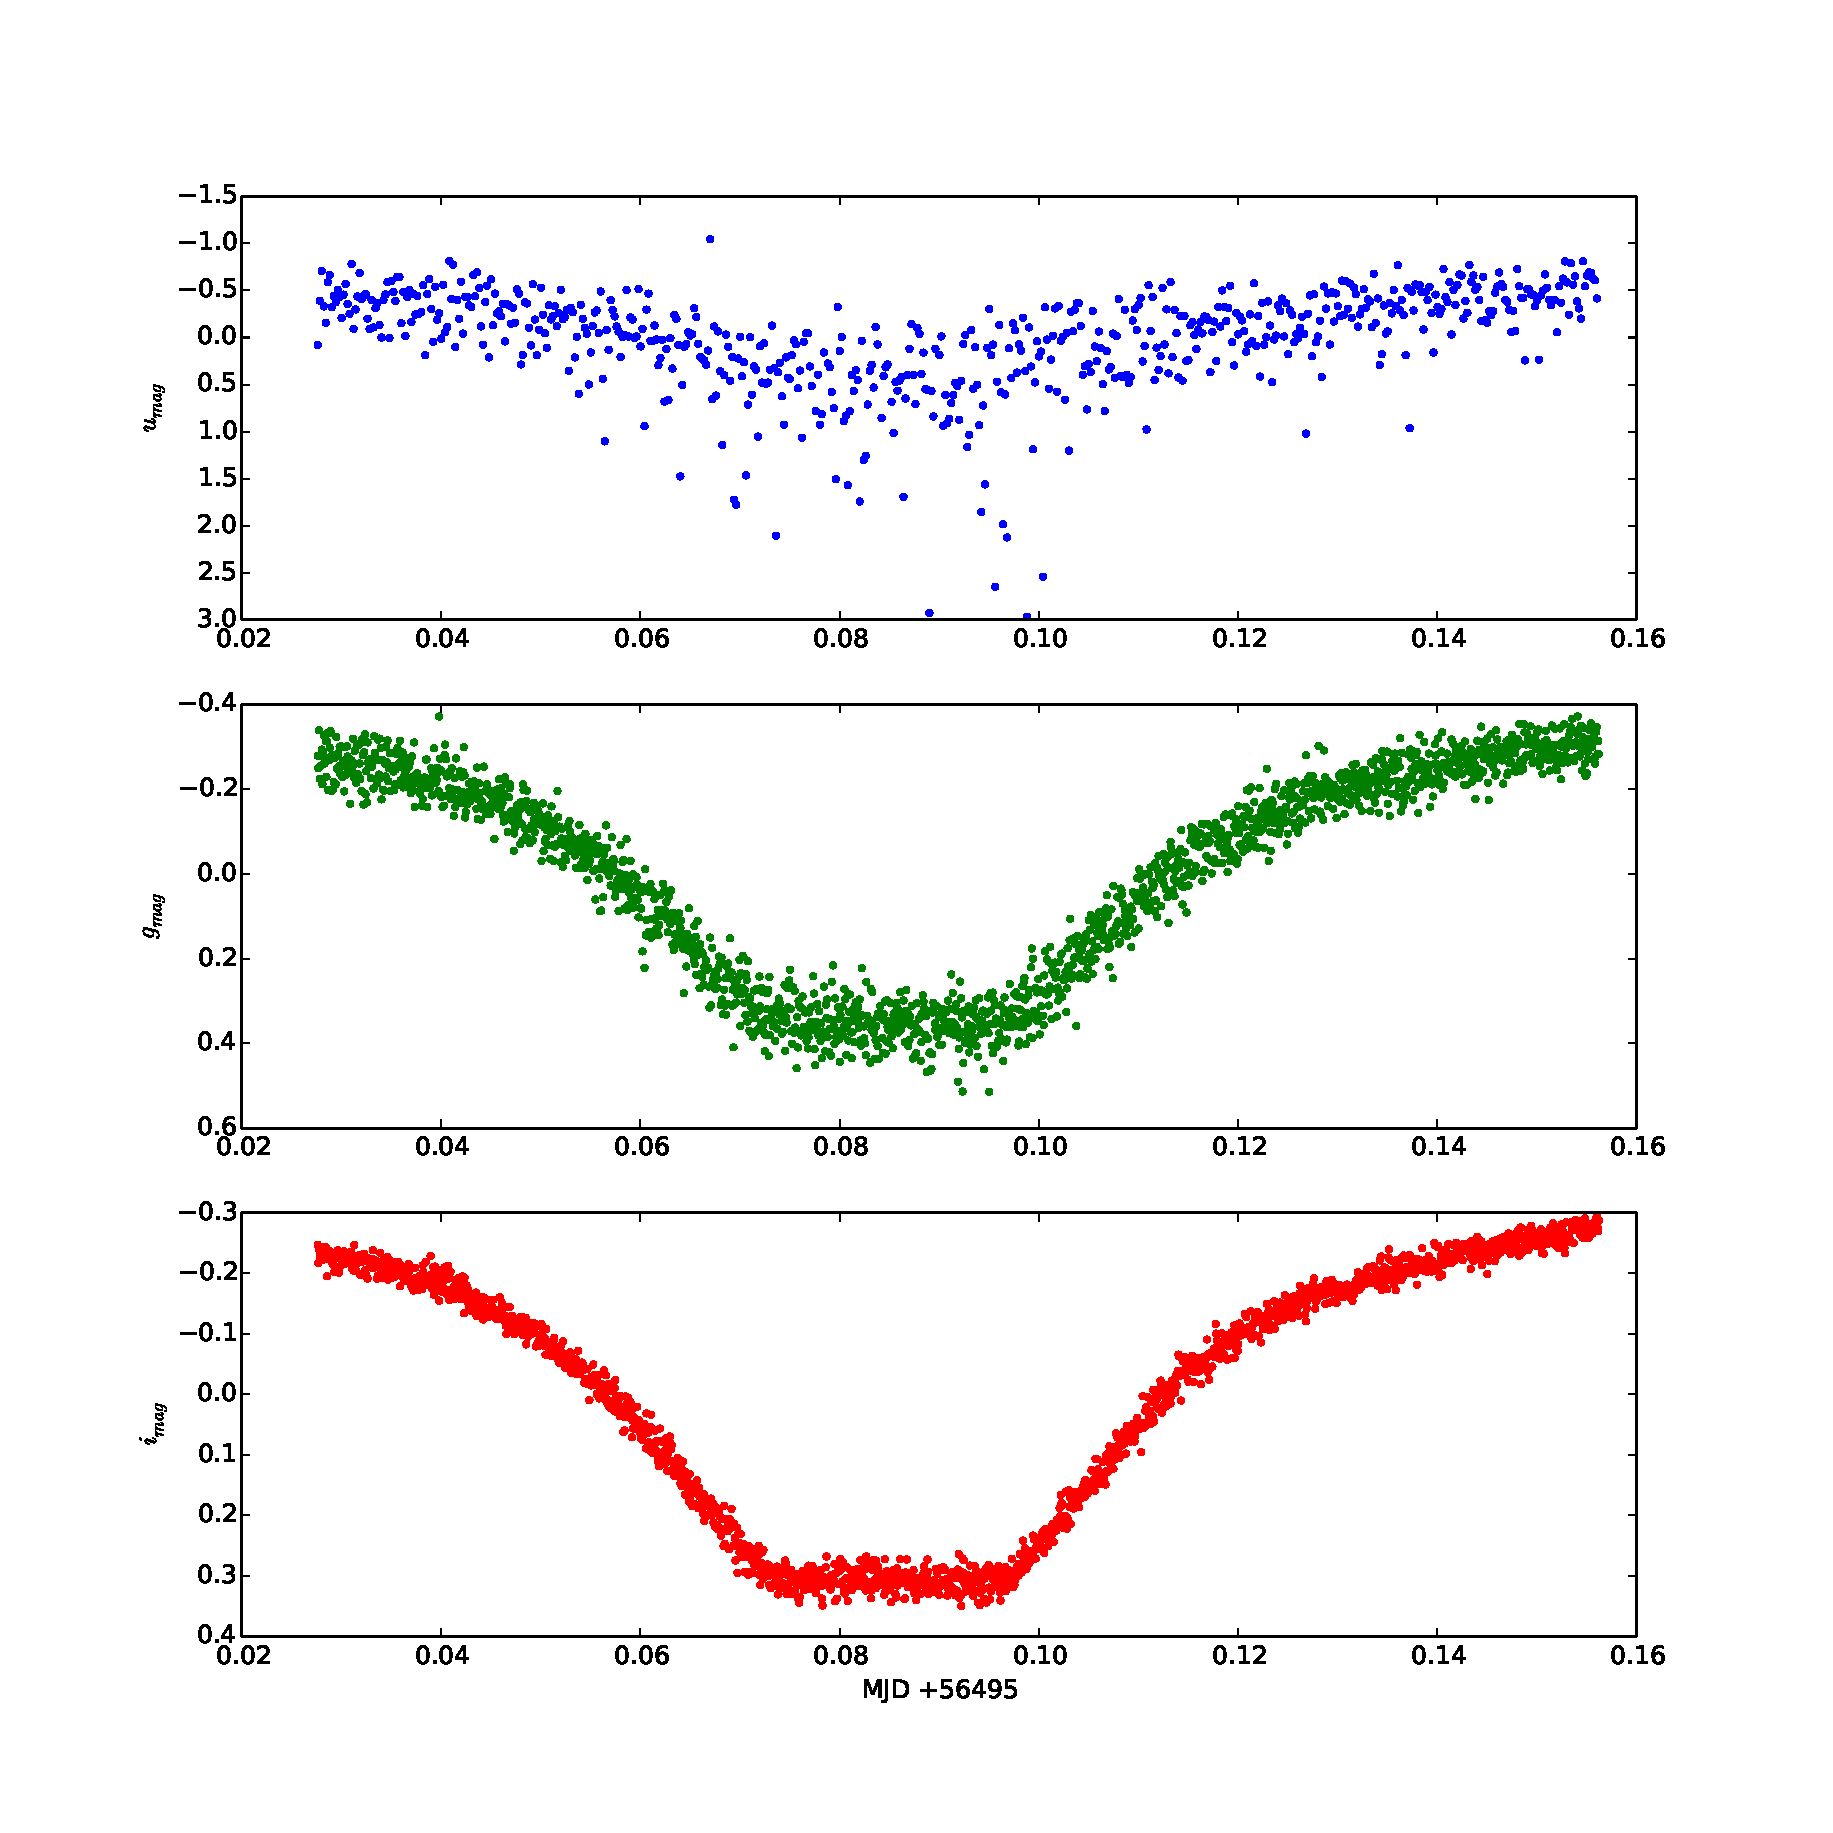
\includegraphics[width=120mm]{images/2013-07-21-run011-162_lightcurve.eps} \\
  The light curve of this object includes a primary eclipse of the object. Since the primary eclipse has a 'flat-bottom' we can conclude that this eclipse is total (ie that the primary is completely obscured by the secondary during the eclipse. This also means that the primary has a small diameter than the secondary. The primary eclipse duration is xxx minutes. The depth of the eclipse is about 0.7 magnitudes which corresponds to an actual drop in flux of 50\%. 

  It is notable that the ingress and the egress demonstrates broad 'wings' suggesting that the object being eclipsed (primary) is extended and the shape of the curve suggest tidal distortion of the secondary.

  Although the object is in a Kepler field and is, in fact, close to KOI-1546, a search through the Kepler archive \footnote{\url{https://archive.stsci.edu/kepler/data_search/search.php}} reveals that it is not listed. This is probably because the object is too faint and the data for this object has not been downloaded. 

\newpage
\subsection{Intrinsic variables}

  \begin{tabular}{l l}
  Classification & $\delta$ Scuti \\
  ObjectID & 2013-07-21-run010-23 \\
  Pixel position & (54, 362) \\
  RA, DEC & 19:44:19.6, 40:16:43.7 (J2000) \\
  URL: & \small \url{http://deneb.astro.warwick.ac.uk/phrnaw/sitedev/2013-07-21/run010.html} \\
       & 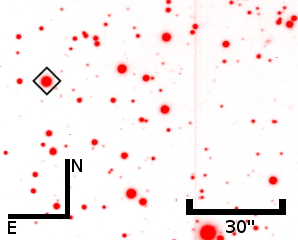
\includegraphics[width=60mm]{images/2013-07-21-run010-23.png} \\
  \end{tabular}
  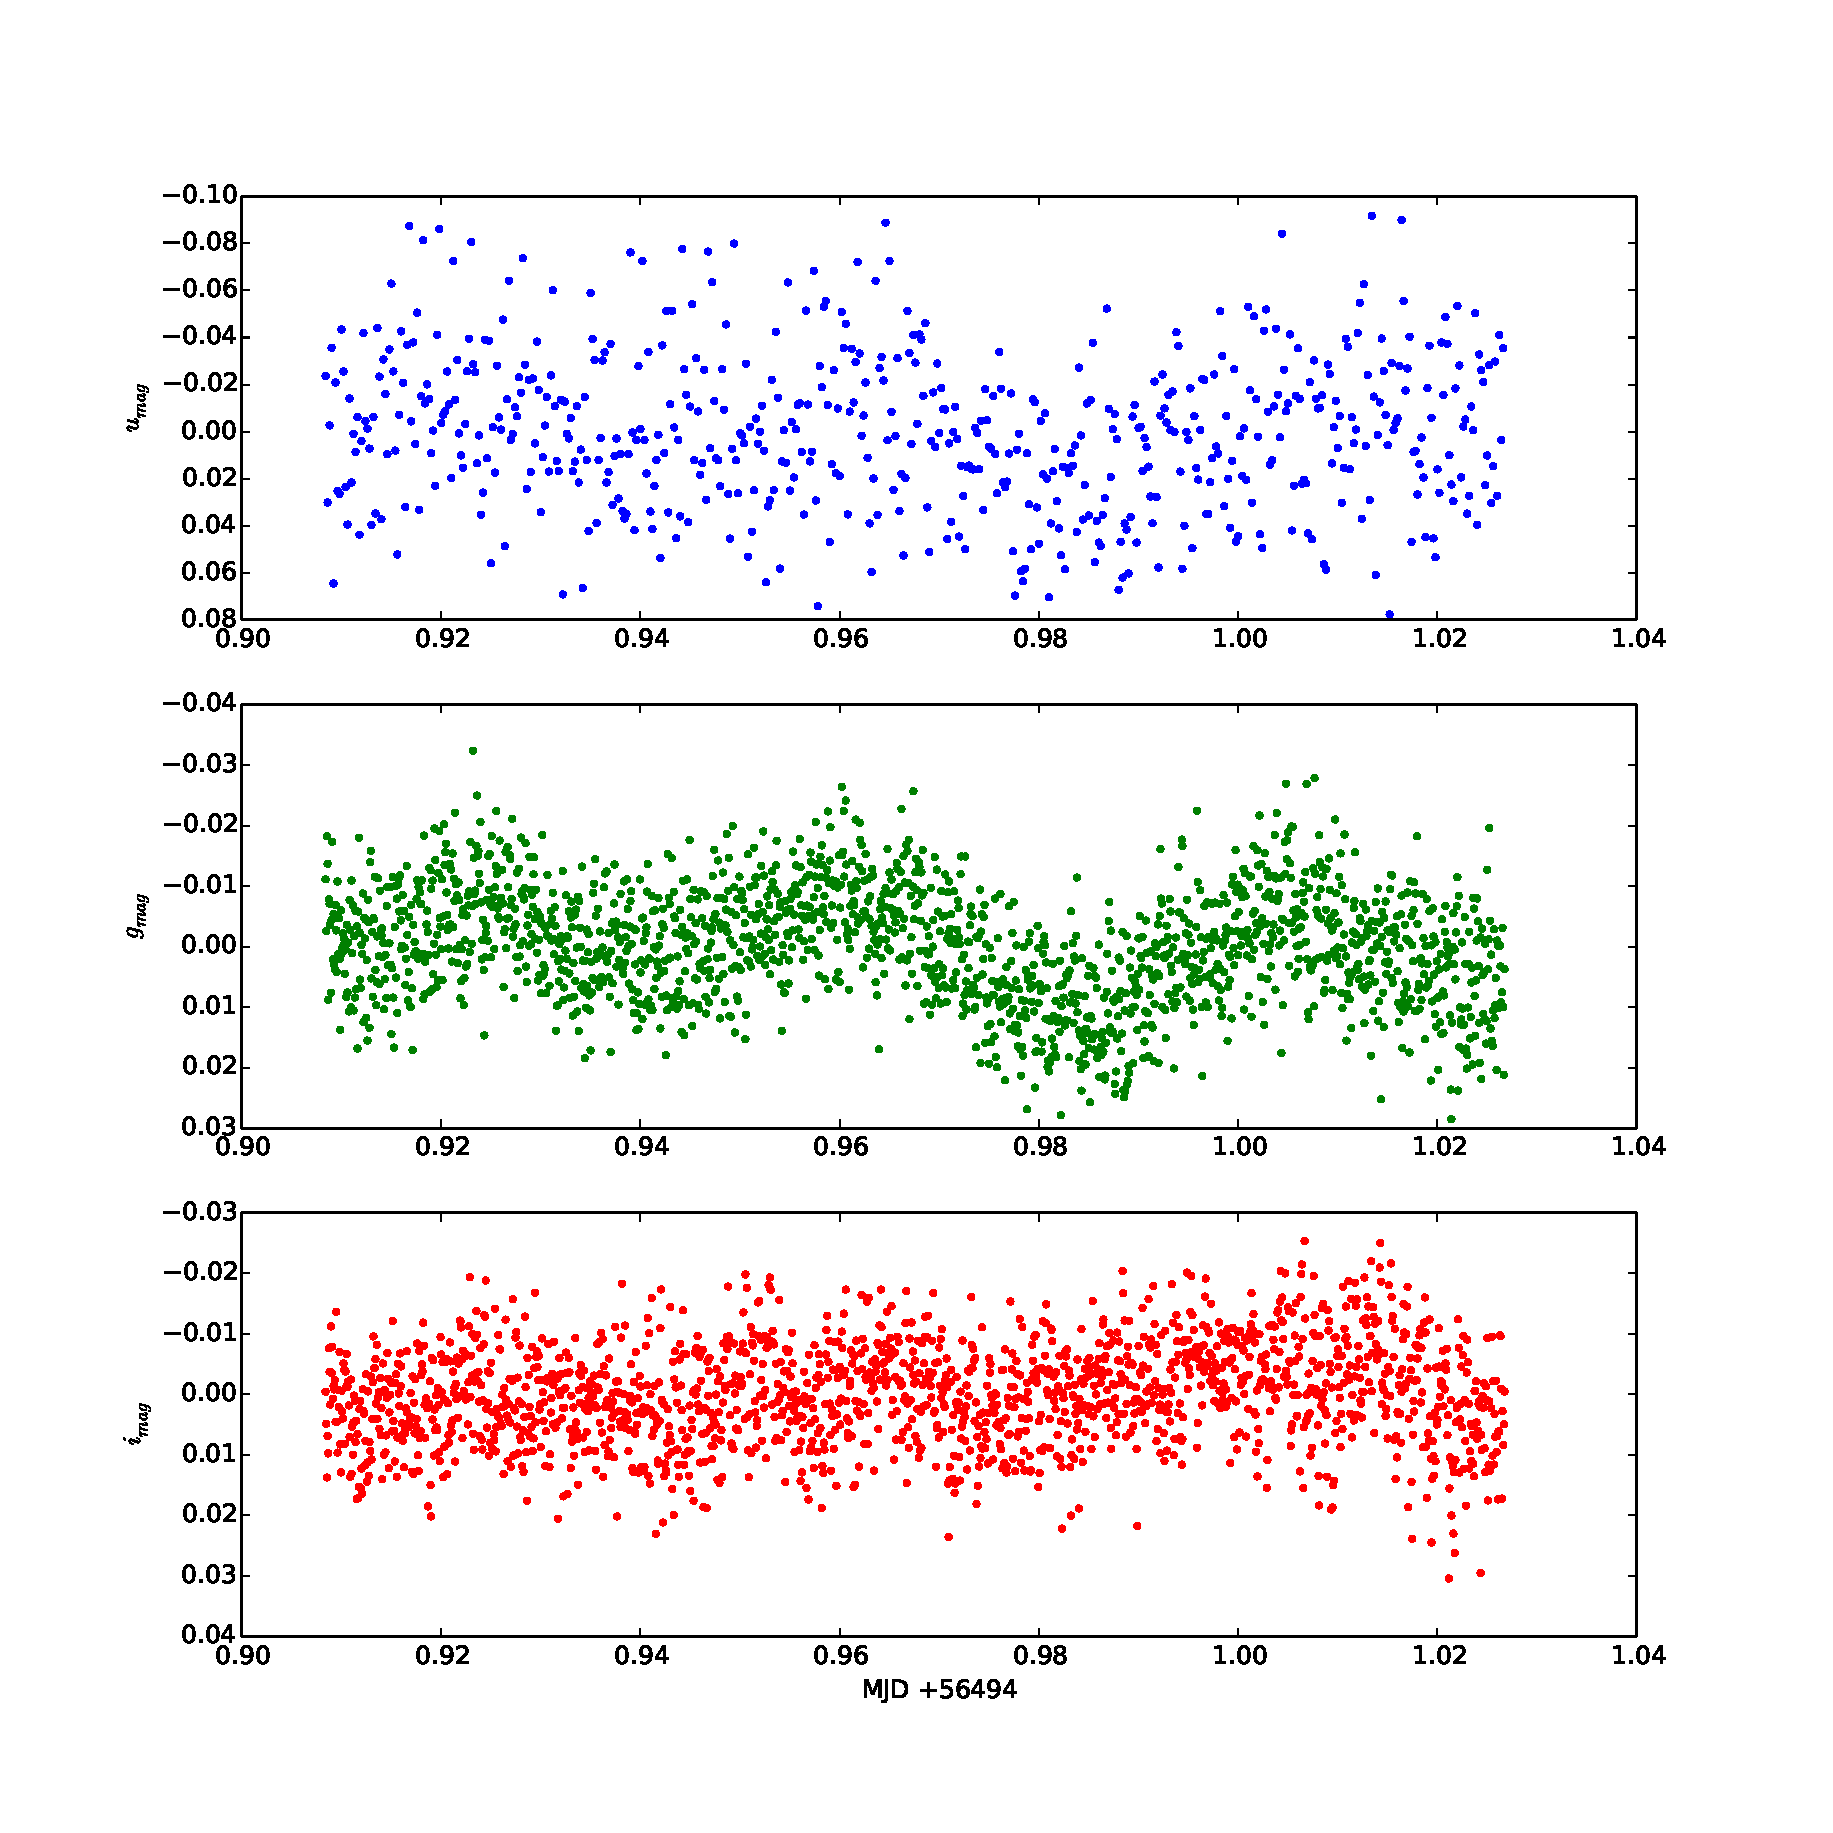
\includegraphics[width=120mm]{images/2013-07-21-run010-23_lightcurve.eps} \\
  This object was found on a run that included the exoplanet host, KIC5115978, which has at least one planet, \cite{KIC5115978}. The new variable is located about 6 arc minutes away from the target. A search of the Kepler data archive \footnote{\url{http://archive.stsci.edu/kepler/kepler_fov/search.php}} gives no results for this object. Unfortunately this object is not in a Kepler field of view, but lies in a position that does not fall on the Kepler CCD. We have no further photometry for this object. 

  There is evidence that the colour is varying in phase with magnitude, most noticeably in $g-i$. The lightcurve is the shape we would expect, with a steeper slope during increasing flux than decreasing. This object is an A or F class star, as would be expected for δ-Scuties. The period is approximately 0.04 days, consistent with the expected range 0.03-0.3 days.


\newpage
\subsection{Near Earth objects}

  \begin{tabular}{l l}
  Classification & Asteroid: 1998 SU139 \\
  ObjectID & 2011-08-26-run014-110 \\
  Pixel position & start: (217, 9), end: (505, 54) \\
  Distance travelled & 291 pixels or 101" \\
  Field scale & 0.35"/pixel \\
  Duration of run & 12355s (3.43 hours) \\
  Tangential angular velocity & 0.495"/minute or 29.68"/hour\\ 
  RA, DEC & MJD=55800.038, 20:51:12, -08:31:25 (J2000) \\
  URL: & \small \url{http://deneb.astro.warwick.ac.uk/phrnaw/sitedev/2011-08-26/run014.html} \\
  \end{tabular}
  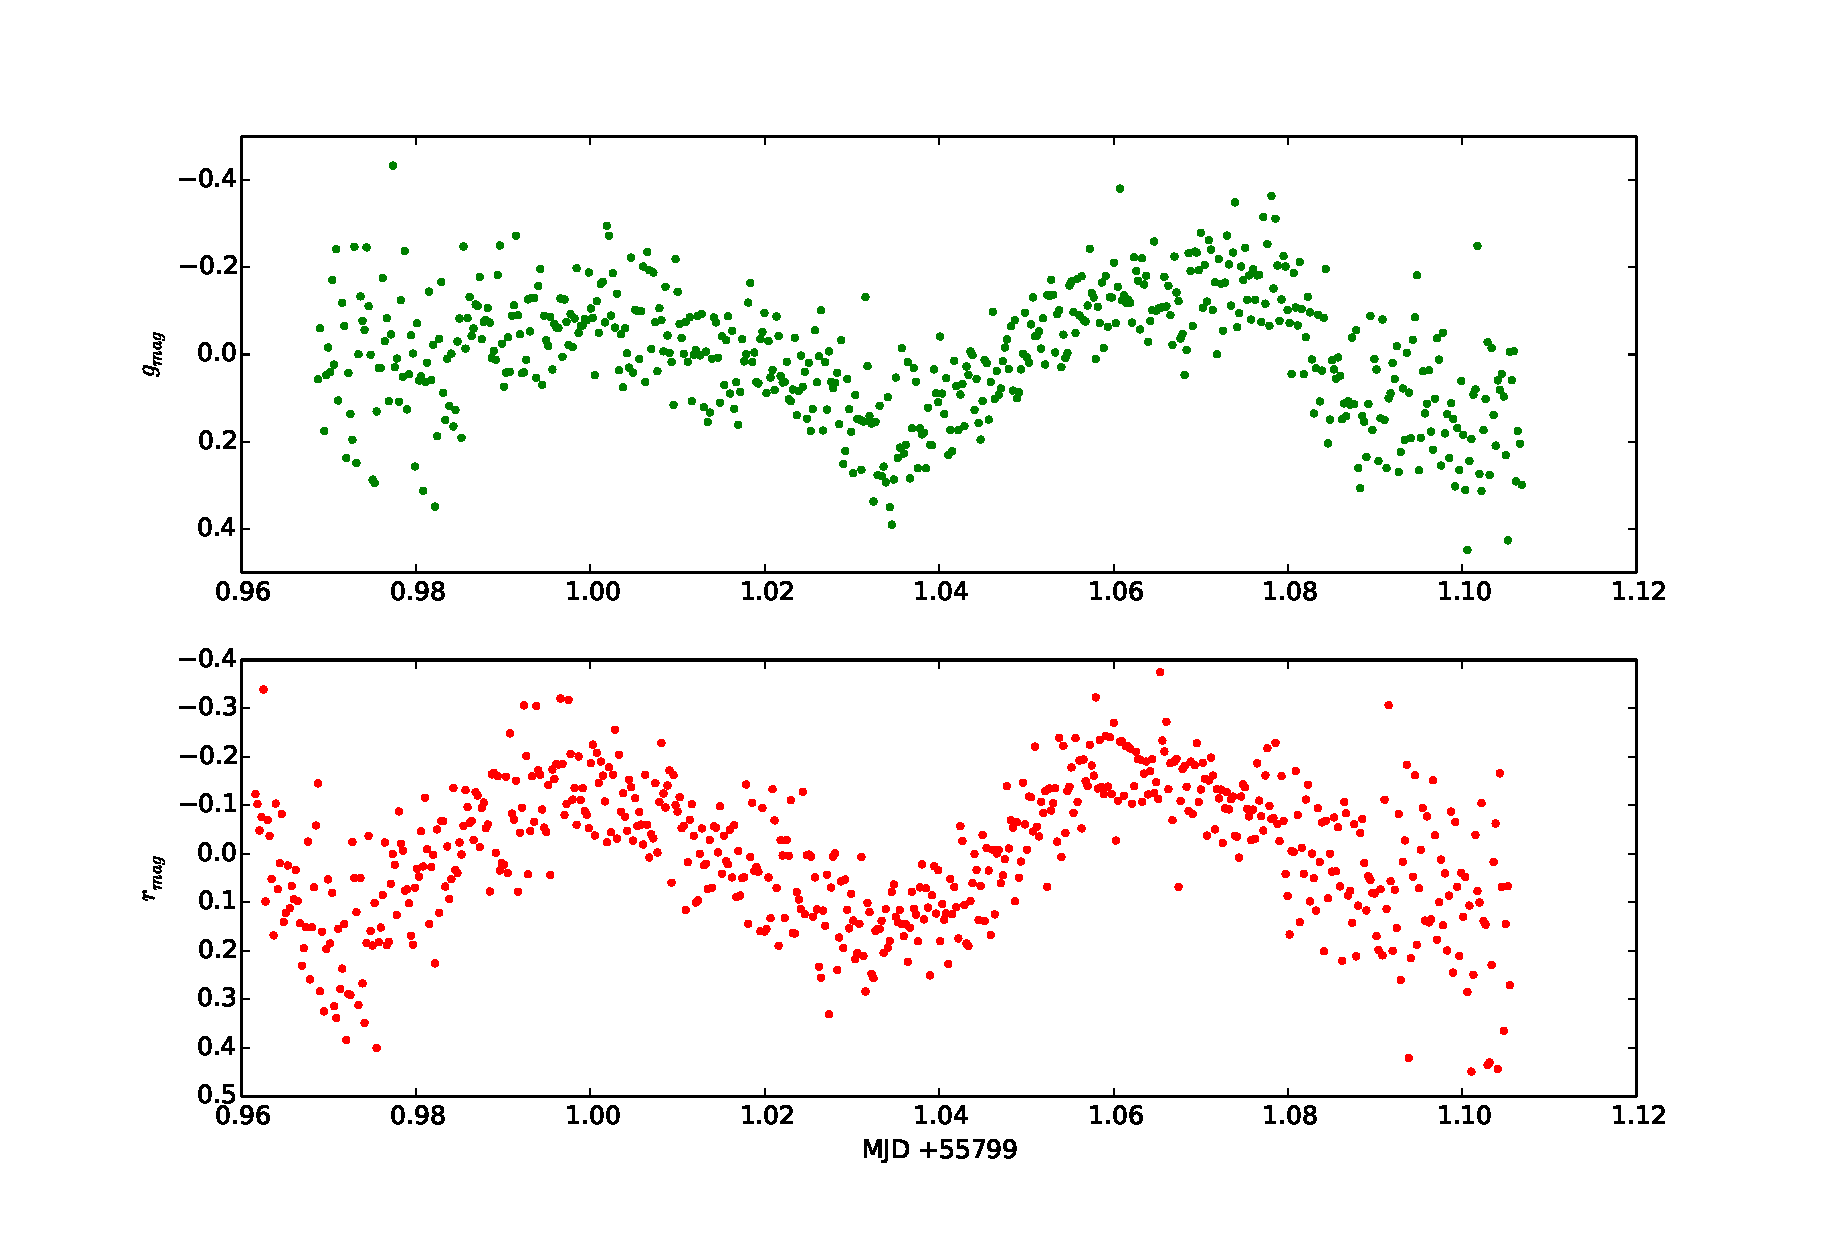
\includegraphics[width=140mm]{images/2011-08-26-run014-110-lightcurve.eps} \\
  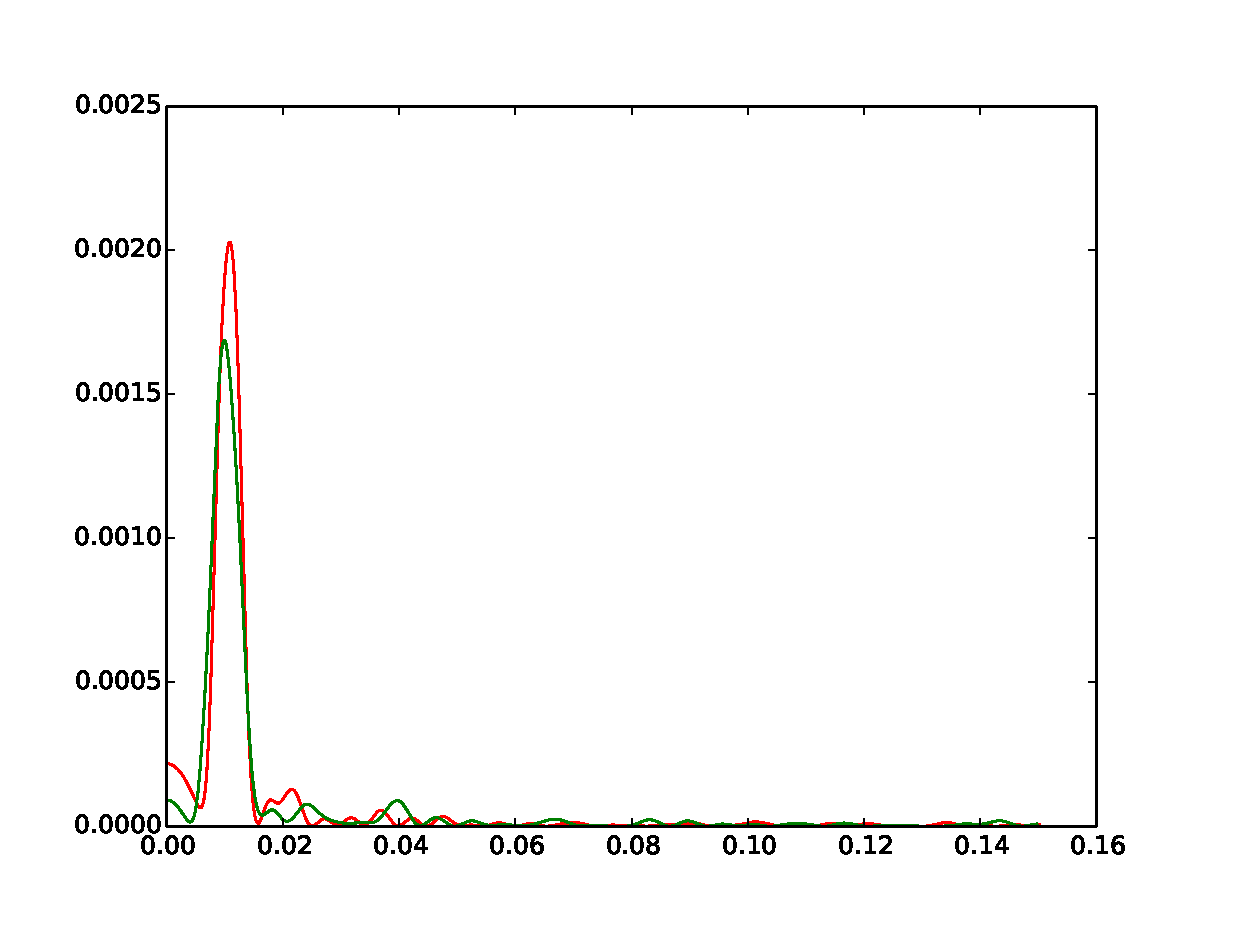
\includegraphics[width=90mm]{images/asteroid_pgram.eps} \\

  The light curve of this object displays a clear sinusoid which must be caused by variations in reflected sunlight that is modulated as the object rotates. A periodogram of these data peaks at a frequency of $0.0108 minutes^{-1}$ (a spin period of $1.53$ hours) for the 'i' filter and $0.0098 minutes^{-1}$ (a spin period of $1.70$ hours) for the 'g' filter. This assumes that one period in the light curve is equal to exactly one rotation of the asteroid. This might not be true if the asteroid has several light and dark patches on its surface. 

  Rotation of asteroids is driven by a process known as the YORP effect, (\cite{yorpeffect}). 

  A look-up using the \emph{NEOChecker} tool on the website of the IAU's Minor Planet Center \footnote{http://www.minorplanetcenter.net/cgi-bin/checkneo.cgi} returns a result for this candidate as, most probably, asteroid \emph{1998 SU139}. The world coordinates reported by the tool differed from our own determination by about 6.5'. 

  There is a clear relationship between the size of the asteroid and the minimum spin period. Observationally, it can be shown that, for an asteroid with a diameter greater than 250 metres, the spin period cannot be less than 2.33 hours, \cite{Jacobson2014}. The theoretical reasoning for this 'spin cut-off'  is that, assuming these asteroids are 'rubble-piles' then, above certain angular velocity, the centrifugal forces pulling the rubble pile apart will be stronger than the gravitational forces holding it together and the rubble pile will break up. At the moment, only two asteroids have been found that are exceptions to this rule, \emph{2001 OE84} and \emph{2005 UW163} with periods of 0.486 and 1.290 hours respectively, \cite{Chang2014}. 

  There are several more unconfirmed super-fast rotators (SFR) asteroids reported by \cite{Masiero2009} and \cite{Dermawan2011}. Since these objects have low brightness and fast rotation, periods have not yet been accurately determined. Many of the light curves only have few tens of data points. The fact that we have managed to determine a spin period for this object demonstrated the fact that ULTRACAM is a suitable instrument to use for follow up observations of these other candidates.  

  The diameter of the asteroid can be estimated by using its absolute magnitude $H$ and an assumption for the albedo $p$ using the formula, adapted from \cite{Jewitt2013}

  $D = \frac{1130}{\sqrt{p}}10^{-H/5} $

  We have taken $H = 15.2$ from the JPL Small-Body Database \footnote{http://ssd.jpl.nasa.gov/sbdb.cgi} and assumed an albedo of $ p = 0.297$ for a V-type asteroid. This gives a diameter, $D = 1.89 km$ for this asteroid. 

  If our period is correct, this could mean that we have discovered a new member of this rare, fast rotator class of asteroid. 

  \newpage

  \begin{tabular}{l l}
  Classification & Asteroid: 9108 Toruyusa (1997 AZ6) [offset of 7 arc minutes from the computed ephemeris]\\
  ObjectID & 2009-01-04-run024-61 \\
  Pixel position & start: (137, 422), end: (226, 447) \\
  Distance travelled & 92 pixels or 32" \\
  Field scale & 0.35"/pixel \\
  Duration of run & 3221s (53.7 minutes) \\
  Tangential angular velocity & 0.596"/minute or 35"/hour\\ 
  RA, DEC & MJD=54836.26642, 08:04:52.3 +16:18:10.6 (J2000) \\
  URL: & \small \url{http://deneb.astro.warwick.ac.uk/phrnaw/sitedev/2009-01-04/run024.html} \\
       & 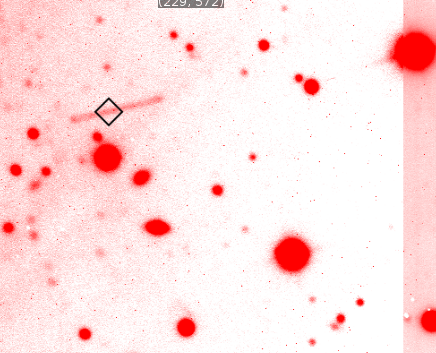
\includegraphics[width=60mm]{images/2009-01-04-run024-61.png} \\
  \end{tabular}

  Using the NEOChecker \footnote{http://www.minorplanetcenter.net/cgi-bin/checkneo.cgi} tool, the object detected in this run appears to be a well known asteroid, 9108 Toruyusa. The light curve, which lasts approximately 1 hour shows no significant variation and it has not been possible to determine a spin period for this asteroid.  

  
